
\subsection{Voorpagina}\label{voorpagina}

\subsubsection{Grid}

De template van de website bestaat uit een grid, een soort geraamte. Het grid is opgebouwd uit verschillende regio's. In elke regio kunnen blokken geplaatst worden. In de paragraaf \emph{Felix}\seeone{felix} staat beschreven hoe en welke je blokken kunt toevoegen aan een regio. 

\bigskip

\begin{center}
	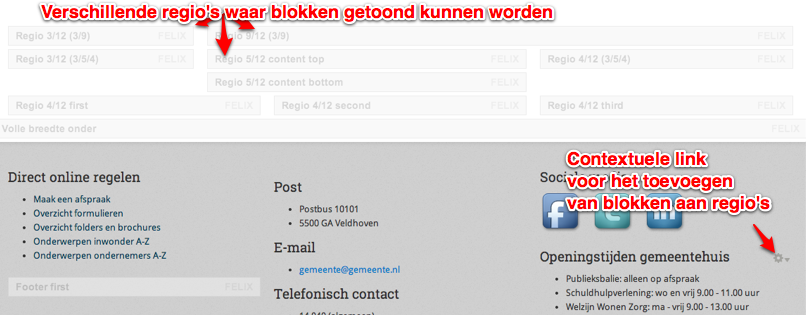
\includegraphics[width=\textwidth]{img/grid1.png}
\end{center}

\subsubsection{Blokken}

In het onderstaande afbeelding worden alle bestaande blokken op voorpagina in het kort toegelicht.

\bigskip

\begin{center}
	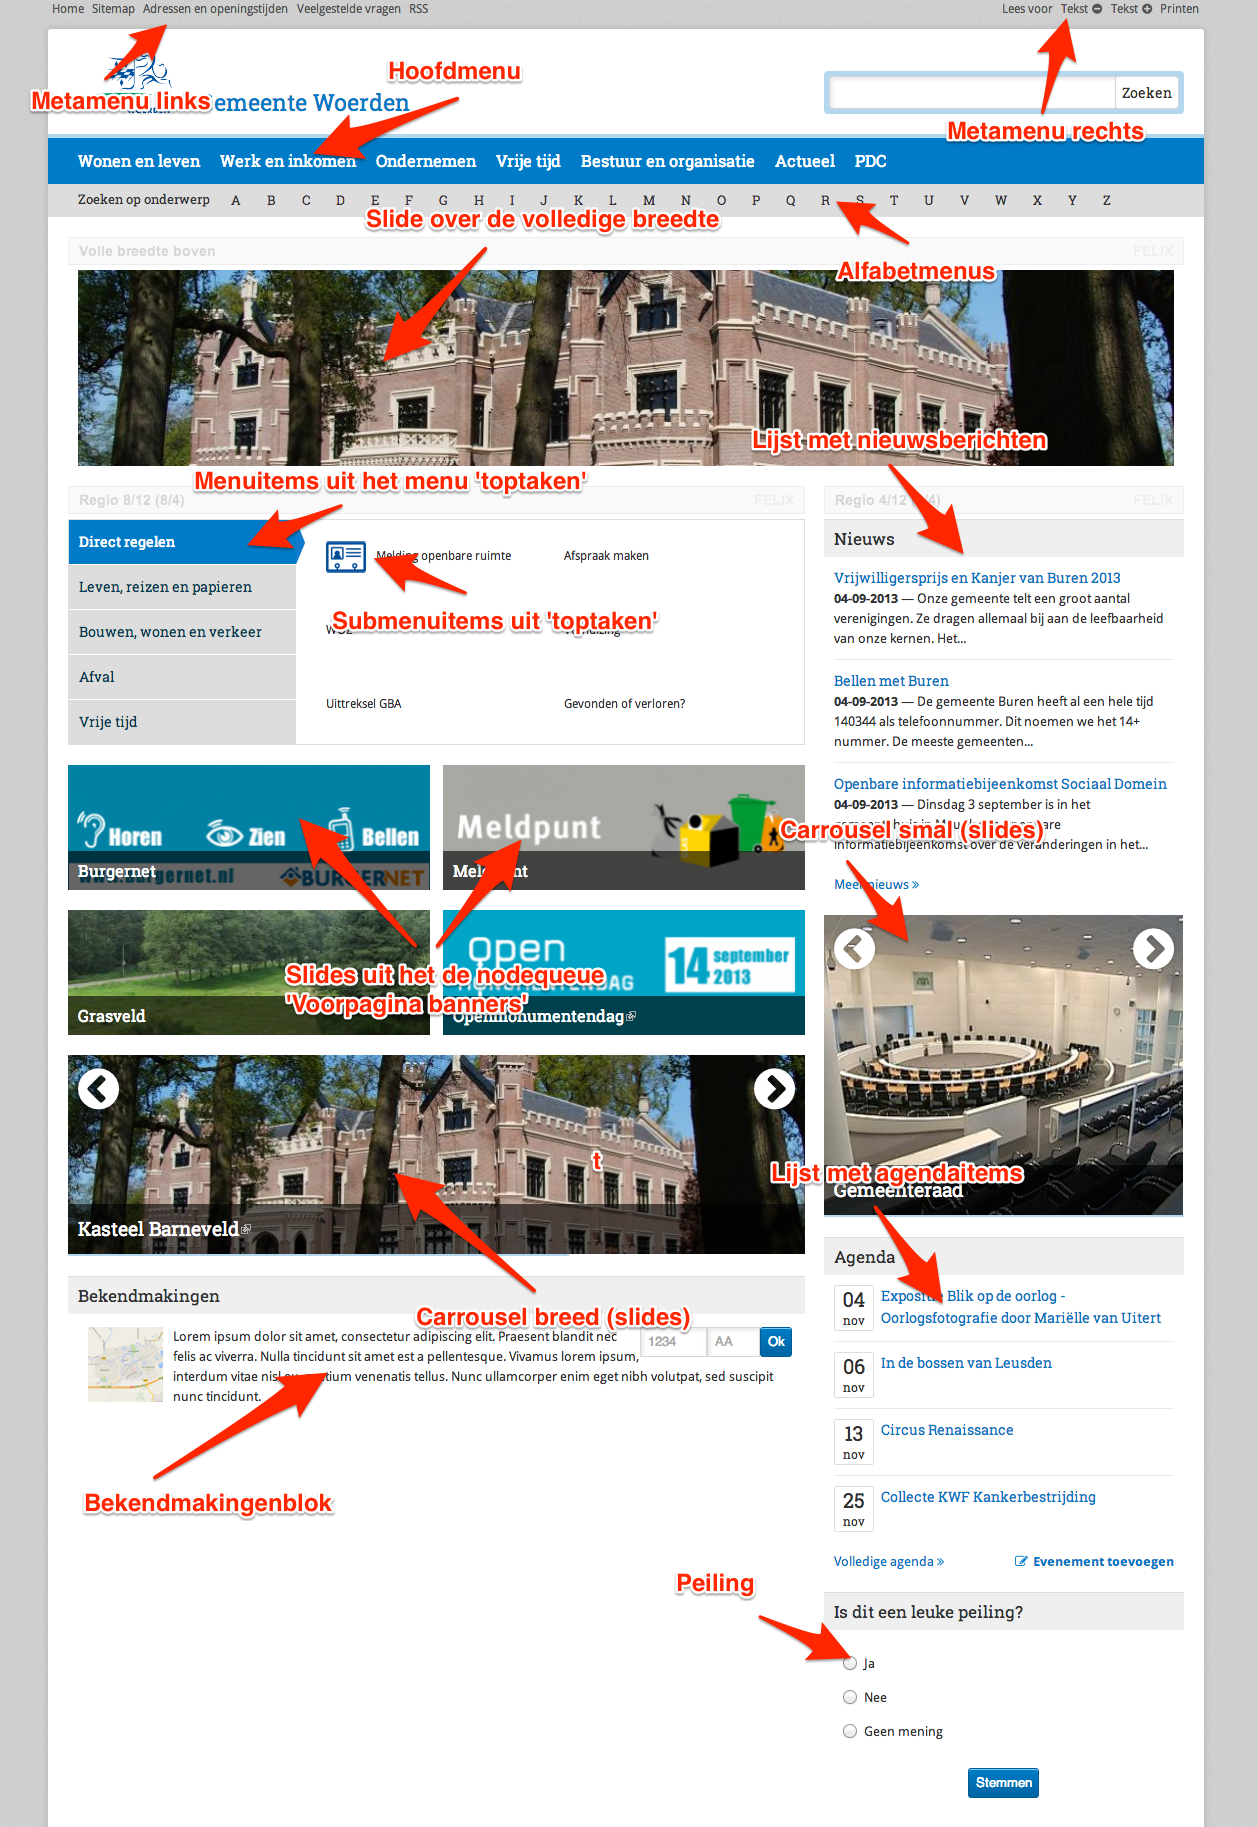
\includegraphics[width=\textwidth]{img/voorpagina.png}
\end{center}

\subsubsection{Footer}

In het onderstaande afbeelding worden alle bestaande blokken in de footer in het kort toegelicht. De footer bestaat uit 3 regio's waar blokken in gezet kunnen worden. De standaard configuratie is links een menu blok "Direct online regelen", in het hoofdstuk \emph{Menu}\seeone{menu} wordt beschreven hoe het menu te bewerken is. In de middenkolom staat blok met redactionele content. In de rechterkolom staan twee blokken; het eerste blok is het Dominion social blok. In paragraaf \emph{Social media}\seeone{socialmedia} staat beschreven hoe deze opties te beheren zijn. Daaronder staat nog een blok met redactionele content. Naast de standaard geconfigureerde blokken zijn in de drie regio's ook nog Felix blokken te zetten. 

\bigskip

\begin{center}
	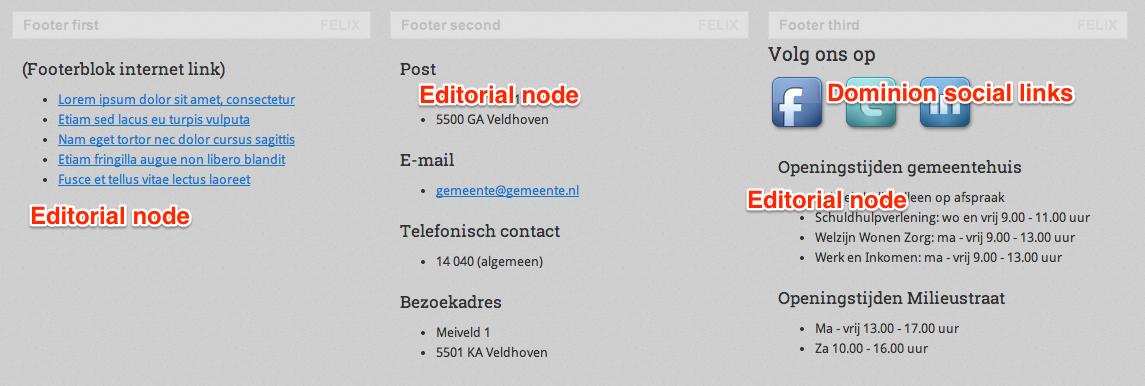
\includegraphics[width=\textwidth]{img/voorpagina3.png}
\end{center}